\renewcommand{\tmpwidth}{18mm}
\setlength{\tabcolsep}{1pt}


\twocolumn[
\begin{@twocolumnfalse}
{
\begin{center}
\begin{tabular}{m{20mm}m{2mm} cccc c cccc}

Original & 
&
&&& \parbox[c]{\tmpwidth}{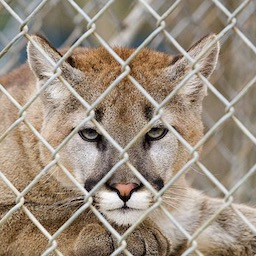
\includegraphics[width=\tmpwidth]{figures/analysis/cougar.jpeg}} &
&
&&& \parbox[c]{\tmpwidth}{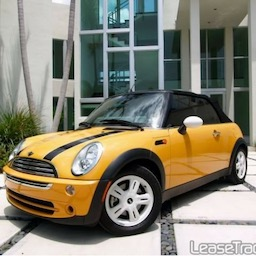
\includegraphics[width=\tmpwidth]{figures/analysis/car.jpeg}} 
\\
\\[-4pt]
&
& Mask 95\% & Mask 90\% & Mask 85\% & Mask 75\% &
& Mask 95\% & Mask 90\% & Mask 85\% & Mask 75\% 
\\ 
\parbox[l]{15mm}{\small{Example Input Mask}} &
&
\parbox[c]{\tmpwidth}{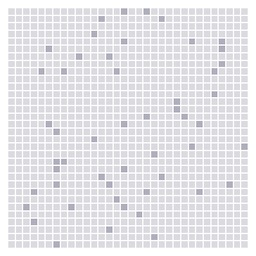
\includegraphics[width=\tmpwidth]{figures/analysis/000286_39_mask03_95.jpeg}}&
\parbox[c]{\tmpwidth}{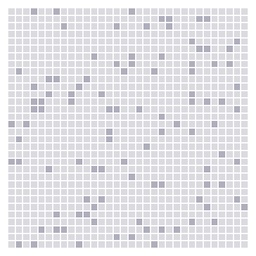
\includegraphics[width=\tmpwidth]{figures/analysis/000286_0_mask01_90.jpeg}}&
\parbox[c]{\tmpwidth}{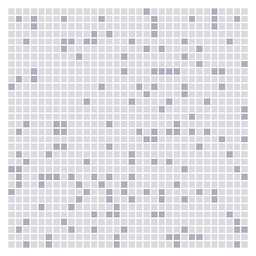
\includegraphics[width=\tmpwidth]{figures/analysis/000286_2_mask_01_85.jpeg}}&
\parbox[c]{\tmpwidth}{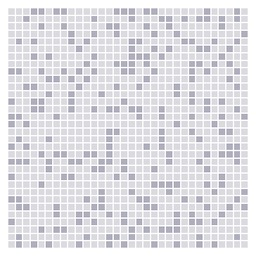
\includegraphics[width=\tmpwidth]{figures/analysis/000286_0_mask03_75.jpeg}}&
&
\parbox[c]{\tmpwidth}{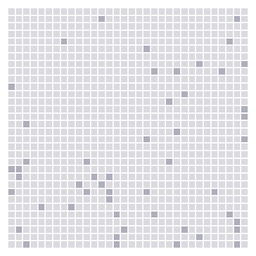
\includegraphics[width=\tmpwidth]{figures/analysis/000511_2_mask_95.jpeg}}&
\parbox[c]{\tmpwidth}{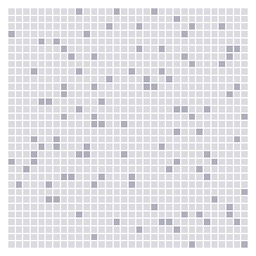
\includegraphics[width=\tmpwidth]{figures/analysis/000511_0_mask_90.jpeg}}&
\parbox[c]{\tmpwidth}{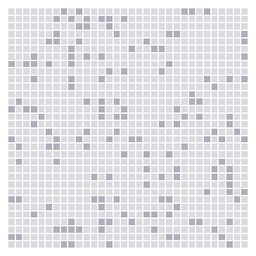
\includegraphics[width=\tmpwidth]{figures/analysis/000511_5_mask_85.jpeg}}&
\parbox[c]{\tmpwidth}{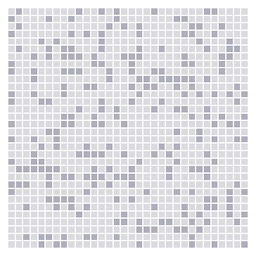
\includegraphics[width=\tmpwidth]{figures/analysis/000511_0_mask_75.jpeg}}

\\
\parbox[l]{15mm}{\small{Reconstruction Sample}} &
&
\parbox[c]{\tmpwidth}{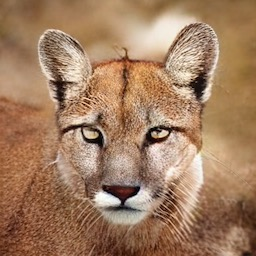
\includegraphics[width=\tmpwidth]{figures/analysis/000286_39_output_95.jpeg}}&
\parbox[c]{\tmpwidth}{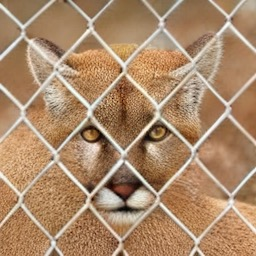
\includegraphics[width=\tmpwidth]{figures/analysis/000286_0_output_90.jpeg}}&
\parbox[c]{\tmpwidth}{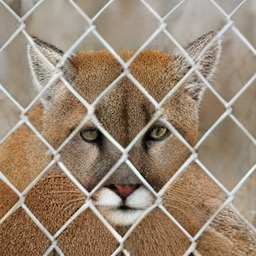
\includegraphics[width=\tmpwidth]{figures/analysis/cougar_85.jpeg}}&
\parbox[c]{\tmpwidth}{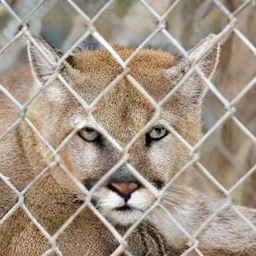
\includegraphics[width=\tmpwidth]{figures/analysis/cougar_75.jpeg}}&
&
\parbox[c]{\tmpwidth}{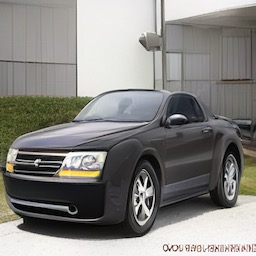
\includegraphics[width=\tmpwidth]{figures/analysis/car_95.jpeg}}&
\parbox[c]{\tmpwidth}{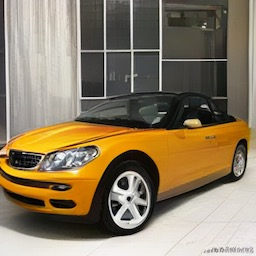
\includegraphics[width=\tmpwidth]{figures/analysis/car_90.jpeg}}&
\parbox[c]{\tmpwidth}{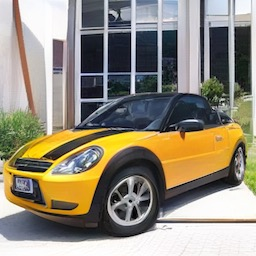
\includegraphics[width=\tmpwidth]{figures/analysis/car_85.jpeg}}&
\parbox[c]{\tmpwidth}{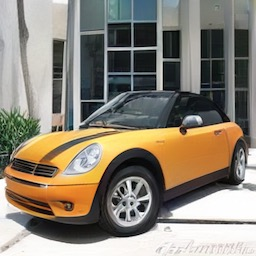
\includegraphics[width=\tmpwidth]{figures/analysis/car_75.jpeg}}

\\
\parbox[l]{20mm}{\small{Median of $100$ Samples}}
 & 
&
\parbox[c]{\tmpwidth}{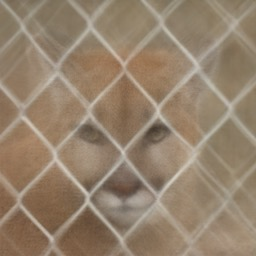
\includegraphics[width=\tmpwidth]{figures/analysis/why_schedule_cougar_statistics_95percent_avg.jpeg}}&
\parbox[c]{\tmpwidth}{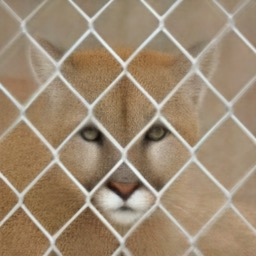
\includegraphics[width=\tmpwidth]{figures/analysis/why_schedule_cougar_statistics_90percent_median.jpeg}}&
\parbox[c]{\tmpwidth}{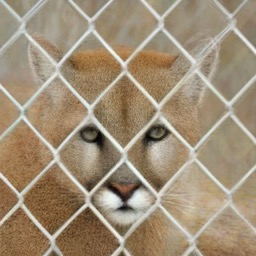
\includegraphics[width=\tmpwidth]{figures/analysis/why_schedule_cougar_85percent_median.jpeg}}&
\parbox[c]{\tmpwidth}{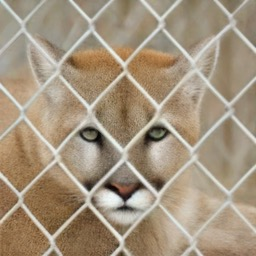
\includegraphics[width=\tmpwidth]{figures/analysis/why_schedule_cougar_statistics_75percent_median.jpeg}}&
&
\parbox[c]{\tmpwidth}{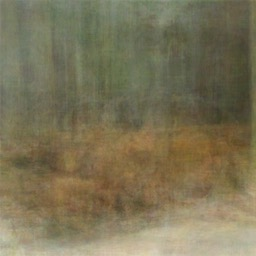
\includegraphics[width=\tmpwidth]{figures/analysis/why_schedule_car_statistics_95percent_median.jpeg}}&
\parbox[c]{\tmpwidth}{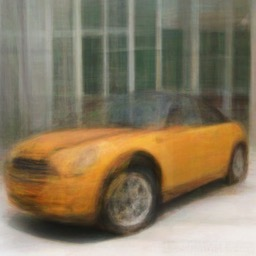
\includegraphics[width=\tmpwidth]{figures/analysis/why_schedule_car_statistics_90percent_median.jpeg}}&
\parbox[c]{\tmpwidth}{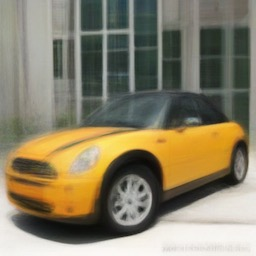
\includegraphics[width=\tmpwidth]{figures/analysis/why_schedule_car_statistics_85percent_median.jpeg}}&
\parbox[c]{\tmpwidth}{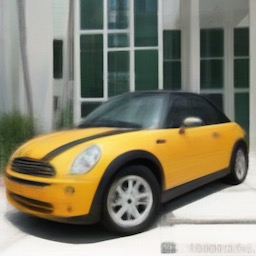
\includegraphics[width=\tmpwidth]{figures/analysis/why_schedule_car_statistics1_75percent_median.jpeg}}
\\
\end{tabular}
\captionof{figure}{\textbf{Examples of \model on Image Reconstruction.} \model takes in masked tokens extracted from original images (row one) using random input masks (row two, with unknown tokens marked in light gray), and outputs reconstructed images (row three). We then randomly sample 100 masks with the same mask ratio, and illustrate the median of the 100 reconstructed samples in row four.}
% The sharpness of the median may be interpreted as the consensus among the reconstruction samples.}
\label{fig:supp_reconstruction}
\end{center}
\vspace{10mm}
}
\end{@twocolumnfalse}
]